\chapter{Feasibility Study of a Pixelated LArTPC for the \dune Near Detector}
\label{chap:dune-nd}

With \AC\ selected as  the \lar\ component of the \dune\ near detector, there were two main question that needed to be addressed:
\begin{enumerate}
	\item Is a pixelated \lartpc\ feasible?
	\item Can the \lar\ detector handle the high rates?
\end{enumerate}
Number one is addressed in Chapter~\ref{chap:viper}.
This chapter will address question number two.


\section{The High-Multiplicity Environment of the \dune\ Near Detector}
\label{sec:dune-nd_multiplicity}

One of the main goals of \dune\ is to measure the Dirac CP violation phase $\delta_{\m{CP}}$ provided it has a non-degenerate value.
To reach a $3 \sigma$ sensitivity for a \SI{75}{\percent} coverage of the $\delta_{\m{CP}}$ parameter space, an exposure of \SI{1320}{\kilo\tonne\mega\watt years} is required (see Figure~\ref{fig:dune-nd_cpv-sens}).~\cite{dune2}
Assuming the reference design of a \SI{40}{\kilo\tonne} far detector and a \SI{1}{\mega\watt} beam results in a data taking time of \SI{33}{years}.
Therefore, to make the data taking time shorter, a beam $>\SI{1}{\mega\watt}$ is required.
On the other hand, combining the numbers of the reference design in~\cite{dune2}, the event rate in the near detector amounts to \SI{0.1}{events\per\tonne\per\mega\watt} leading to significant event pile-up.
This number does not include rock events---secondary particles produced by beam neutrino interactions in the surrounding material, entering the detector.

\begin{figure}[htb]
	\centering
	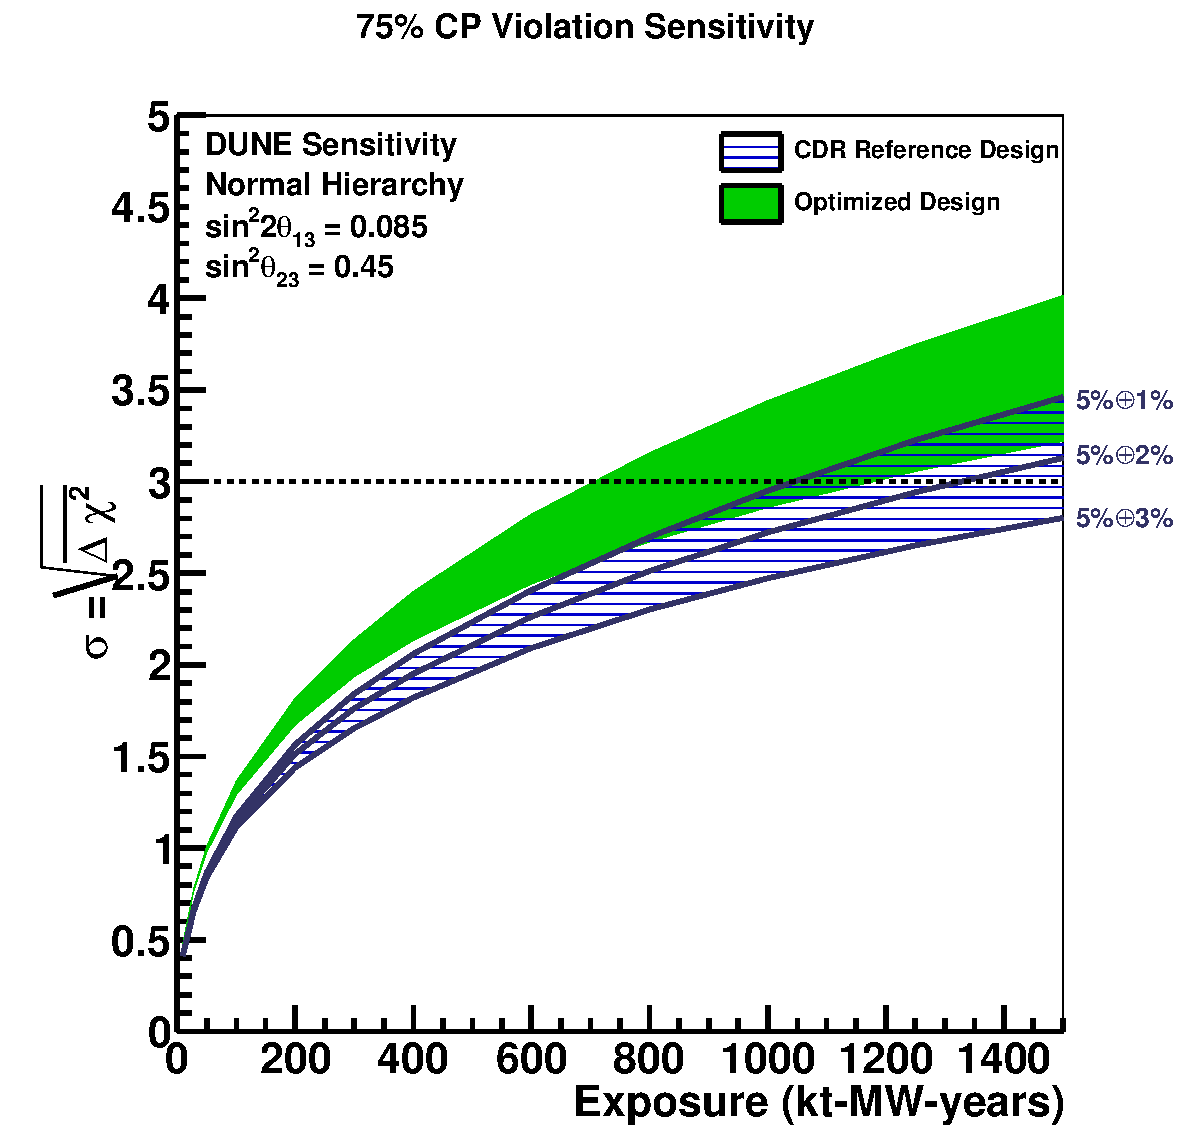
\includegraphics[width=.5\textwidth]{dune-nd/dune_cpv75_exp_syst}
	\caption{Expected sensitivity of \dune\ to discovery of CP violation, i.e.\ $\delta_{\m{CP}} \neq\ 0\ \m{or} \pi$ as a function of exposure in \si{\kilo\tonne\mega\watt years}, assuming equal running in neutrino and antineutrino mode.~\cite{dune2}}
	\label{fig:dune-nd_cpv-sens}
\end{figure}

\section{Simulation}
\label{sec:dune-nd_simulation}

Establishing a simulation of the pixelated readout assists its design and implementation in future detectors, which will be especially important for the physics requirements of those detectors.
An important outcome is the influence of the module walls on reconstruction efficiencies.
They can be regarded as missing pixels in the simulation.
My task is to implement the actual pixel readout into existing simulations of future detectors in the beginning of 2017.
